\section{How to read this guide}

This guide tries to accomodate two needs: first of all, having a handy reference on how to configure the most common services's crypto settings and second of all, explaining a bit, how to chose your own cipher settings.
\vskip 0.5em

System administrators who want to copy \& paste recommendations quickly without spending a lot of time on background reading on cryptography or cryptanalysis can do so, by simply searching for the corresponding section in chapter  \ref{section:PracticalSettings} (``Practical recommendations''). However, for the quick copy \& paste approach it is important to know that this guide assumes users are happy with \textit{cipher String B} which is the baseline and most compatible recommendation that the authors came up with. \textit{Cipher string B} is described in \ref{section:recommendedciphers}.
\textit{Cipher String B} covers the most common use-cases (such as running an e-commerce shop, a private homagepage, a mail server, $ \ldots $)


\vskip 0.5em

While chapter \ref{section:PracticalSettings} is intended to server as a copy \& paste reference, chapter \ref{chapter:Theory} (``Theory'') explains the reasoning behind \textit{cipher string B}. In particular, section \ref{section:CipherSuites} explains how to choose individual cipher strings. We advise the reader to actually read this section and challenge our reasoning in chosing \textit{cipher string B} and to come up with a better  or localized solution.


%We start with some general remarks in sections \ref{section:DH},\ref{section:EllipticCurveCryptography},\ref{section:keylengths} on 


%If you are a system administrator and want to quickly update your services, jump right to section \ref{section:PracticalSettings}. However, we recommend that you take some time and first read through the theory part (chapter \ref{chapter:Theory}), especially section \ref{section:CipherSuites} on how to choose your own cipher string and then adapt the settings in section \ref{section:PracticalSettings} to your own needs.

\vskip 1.5em

\begin{figure}[h]
  \centering
  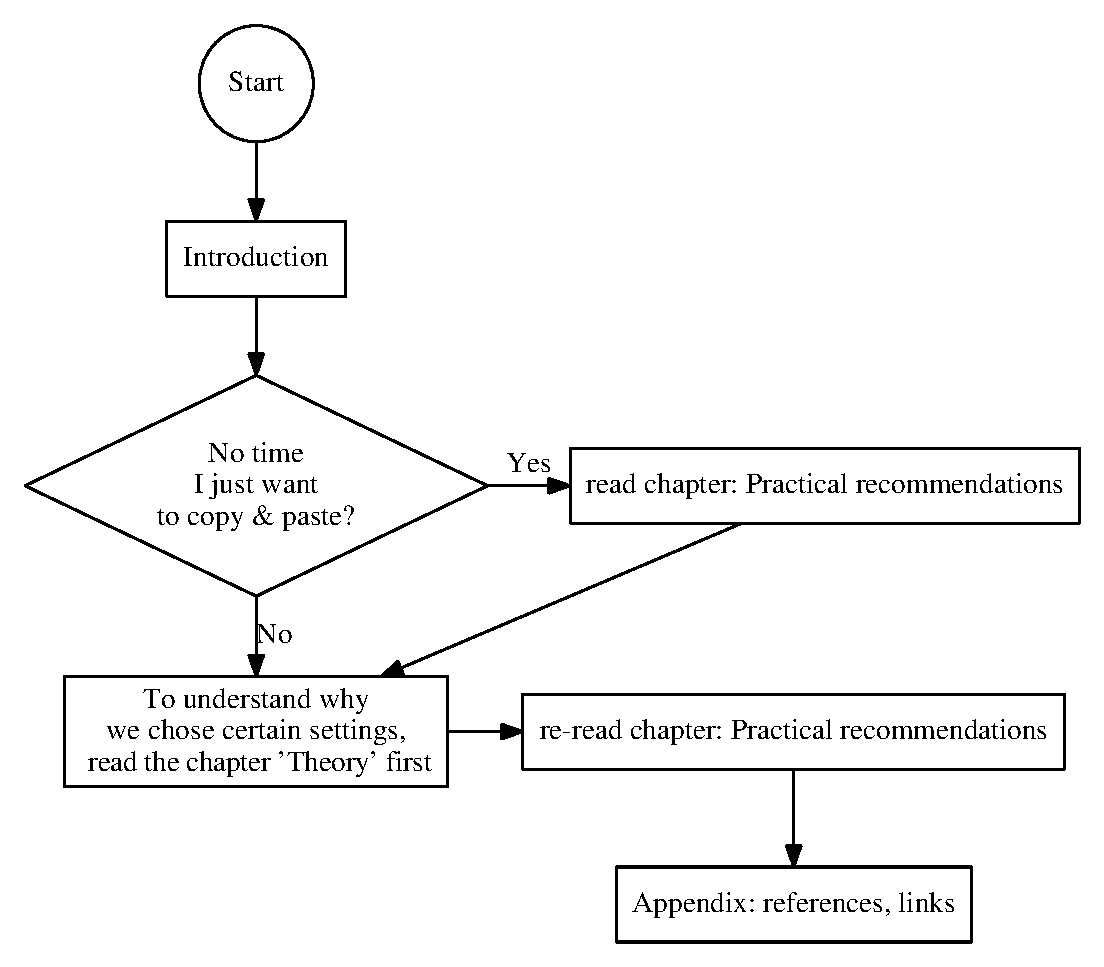
\includegraphics[width=0.55\textwidth]{img/howtoread}
  %\caption{Screenshot of \url{http://www.keylength.com} for 128 bit symmetric key size equivalents}
  \label{fig:howtoread}
\end{figure}

\vskip 2em



